\section{Introduction}
\section{Tools}
\subsection{IDE}
\subsection{Version Control}
% \subsection{Project Management}
\subsection{Database Visualisation}
\subsection{Libraries}
\subsection{Client Side}
% cytoscape
% rxjs?
% material
\subsection{Server Side}
% neomodel
% more ...
\section{Data Processing}
\subsection{Finding Data Source}
% getting xml file from wiki
% looked a platinum god and other data sources (pokemon)
\subsection{Data Extraction}
% using beautiful soup to parse xml
% then using regex to get the important text from each element
\subsection{Cleaning the Data}
%  using regex to strip out tags etc
\subsection{Importing into Database}
% generating CSV files in the correct format to use the data importer tool
\begin{figure}[H]
    \centering
    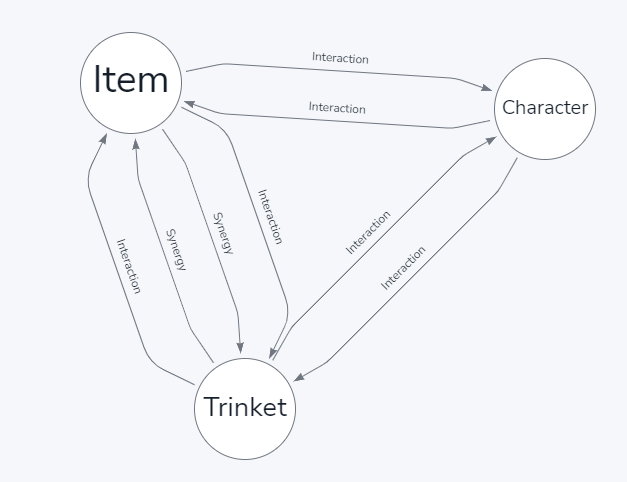
\includegraphics[scale=0.4]{dataImport}
    \caption{Database Model in Neo4j Data Importer}
\end{figure}
\section{Web Stack}
% creating the Django and angular projects and connecting them together
% talk about submodules
\section{Database Interaction}
% creating models
% finding cypher query for getting relationships and all data
% explain that it's really slow
\section{Client Side}
% tables
% using cytoscape to create graphs
% hardcoding files
\section{Conclusion}